\mySection{6.3 Testing Binomial Data -- $H_0:p=p_0$}
%-------------- start slide -------------------------------%{{{ 6.14
\begin{frame}
	% {\S\: 6.3 Testing Binomial Data -- $H_0:p=p_0$}

{\bf Setup:~} Let $X_1=k_1,\cdots,X_n=k_n$ be a` random sample of size $n$ from Bernoulli$(p)$.
$X=\sum_{i=1}^n X_i\sim$ Binomial($n,p$).
We want to test $H_0: p=p_0$.
\pause\vfill
\begin{enumerate}
 \item When $n$ is large, use $Z$ score.  \hfill Large-sample test
 \item Otherwise, use the exact binomial distribution. \hfill Small-sample test
\end{enumerate}
\vfill\pause
\begin{gather*}
\text{$n$ is large}\\
\Updownarrow \\
 0 < np_0 -3\sqrt{np_0(1-p_0)}< np_0 +3\sqrt{np_0(1-p_0)}<n\\
 \Updownarrow \\
 n> 9 \times \max\left(\frac{1-p_0}{p_0},\frac{p_0}{1-p_0}\right).
\end{gather*}
\end{frame}
%-------------- end slide -------------------------------%}}}
%-------------- start slide -------------------------------%{{{ 6.15
\begin{frame}{Large-sample test for $p$}

{\bf Setup:~}
\begin{enumerate}
 \item Let $X_1=k_1,\cdots,X_n=k_n$ be a random sample of size $n$ from Bernoulli$(p)$.
 \item Suppose $n> 9 \max\left(\frac{1-p_0}{p_0},\frac{p_0}{1-p_0}\right)$.
 \item Set $k=k_1+\cdots+k_n$ and $z=\frac{k-np_0}{\sqrt{np_0(1-p_0)}}$.
 \item The level of significance is $\alpha$.
\end{enumerate}
\pause
\vfill
{\bf Test:}\\
\begin{minipage}{0.3\textwidth}
 \[
 \begin{cases}
  H_0: p= p_0 \\
  H_1: p> p_0 \\
 \end{cases}
 \]
 reject $H_0$ if $z\ge z_\alpha$.
\end{minipage}
\hfill
\begin{minipage}{0.3\textwidth}
 \[
 \begin{cases}
  H_0: p= p_0 \\
  H_1: p< p_0 \\
 \end{cases}
 \]
 reject $H_0$ if $z\le -z_\alpha$.
\end{minipage}
\hfill
\begin{minipage}{0.3\textwidth}
 \[
 \begin{cases}
  H_0: p= p_0 \\
  H_1: p\ne p_0 \\
 \end{cases}
  \]
  reject $H_0$ if $|z| \ge z_{\alpha/2}$.
\end{minipage}

\end{frame}
%-------------- end slide -------------------------------%}}}
%-------------- start slide -------------------------------%{{{ 6.16
\begin{frame}{Small-sample test for $p$}
\begin{enumerate}
 \item[E.g.] $n=19$, $p_0=0.85$, $\alpha=0.10$. Find critical region for the two-sided test
 \[
		 \begin{cases}
			H_0: p= p_0 \\
			H_1: p\ne p_0 \\
		 \end{cases}
 \]
 \vfill\pause
 Sol. $19 = n < 9 \times \max\left(\frac{0.85}{0.15},\frac{0.15}{0.85}\right) = 51$, so small sample test. \\[1em]\pause
 By checking the table, the critical region is
 \[
 C = \{k: k\le 13 \quad\text{or}\quad k=19\},
 \]
 so that
 \begin{align*}
	 \alpha &=\PP(X\in C | H_0 \:\: \text{is true}) \\ \pause
 &=\PP(X\le 13|p=0.85)+\PP(X= 19|p=0.85) \\ \pause
 &= 0.099295 \approx 0.10.
 \end{align*}
 \myEnd
\end{enumerate}
\end{frame}
%-------------- end slide -------------------------------%}}}
%-------------- start slide -------------------------------%{{{ 6.17
\begin{frame}
 \begin{center}
  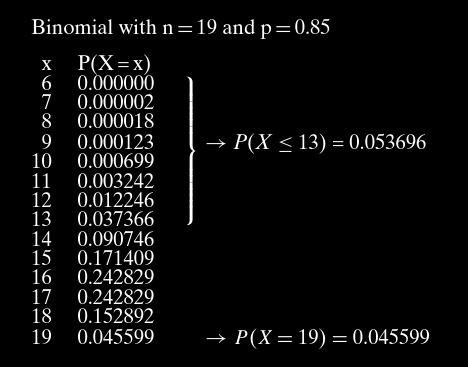
\includegraphics[scale=0.4]{Figure-6-3-1-neg.png}
 \end{center}
\end{frame}
%-------------- end slide -------------------------------%}}}
%-------------- start slide -------------------------------%{{{ 1
\begin{frame}[fragile]
\begin{lstlisting}[language=Python]
# Eg_6-3-1.py
from scipy.stats import binom
n = 19
p = 0.85
rv = binom(n, p)
low = rv.ppf(0.05)
upper = rv.ppf(0.95)
left = round(rv.cdf(low), 6)
right = round(1-rv.cdf(upper), 6)
both = round(rv.cdf(low)+1-rv.cdf(upper), 6)
Results = """\
    The critical regions is less or equal to {low:.0f}, or strictly greater than {upper:.0f}.
		The size of the tail is {left:.6f} and that of the right tail is {right:.6f}.
		Under this critical region, the level of significance is {both:.6f}
""".format(**locals())
print(Results)
\end{lstlisting}
\begin{center}
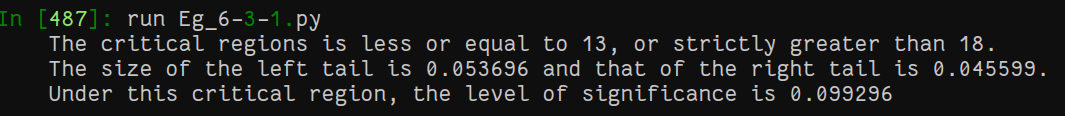
\includegraphics[scale=0.25]{Eg_6-3-1.png}
\end{center}
\end{frame}
%-------------- end slide -------------------------------%}}}
%-------------- start slide -------------------------------%{{{ Guess 54
\begin{frame}[fragile]
\def\guess{54}
\def\ans{0.2421}
  \begin{center}
	$X\sim \text{Binomial}(100,1/2)$
 \bigskip

 \includegraphics[scale=0.3]{Binomial_Jory_\guess.png}
\bigskip
\begin{align*}
  \bbP\left(X\ge \guess\right) = \sum_{n=\guess}^{100} \binom{100}{n} \left(\frac{1}{2}\right)^n \left(\frac{1}{2}\right)^{100-n} = \textcolor{red}{\ans}.
\end{align*}
vs
\begin{align*}
  \bbP\left(\frac{X-50}{\sqrt{100 \times \frac{1}{2}\times \frac{1}{2}}} \ge \frac{\guess-50}{\sqrt{100 \times \frac{1}{2}\times \frac{1}{2}}}\right) \approx
  \bbP\left( Z \ge \frac{4}{5}\right) = \textcolor{green}{0.2119}
\end{align*}
\end{center}
 \end{frame}
%-------------- end slide -------------------------------%}}}

%-------------- start slide -------------------------------%{{{ Guess 60
\begin{frame}[fragile]
\def\guess{60}
\def\ans{0.0284}
  \begin{center}
	$X\sim \text{Binomial}(100,1/2)$
 \bigskip

 \includegraphics[scale=0.3]{Binomial_Jory_\guess.png}
\bigskip
\begin{align*}
  \bbP\left(X\ge \guess\right) = \sum_{n=\guess}^{100} \binom{100}{n} \left(\frac{1}{2}\right)^n \left(\frac{1}{2}\right)^{100-n} = \textcolor{red}{\ans}.
\end{align*}
vs
\begin{align*}
  \bbP\left(\frac{X-50}{\sqrt{100 \times \frac{1}{2}\times \frac{1}{2}}} \ge \frac{\guess-50}{\sqrt{100 \times \frac{1}{2}\times \frac{1}{2}}}\right) \approx
  \bbP\left( Z \ge 2\right) = \textcolor{green}{0.0228}
\end{align*}
\end{center}
 \end{frame}
%-------------- end slide -------------------------------%}}}

